\section{Basics}

\begin{frame}
\frametitle{An introduction to control}
\end{frame}

\begin{frame}
\frametitle{What is control?}
\begin{itemize}
	\item The goal is to find an input (control signal U(s)) such that the process produces the desired output
	\item Open loop control system: the actual output signal has no effect on the control action
\begin{figure}
\centering
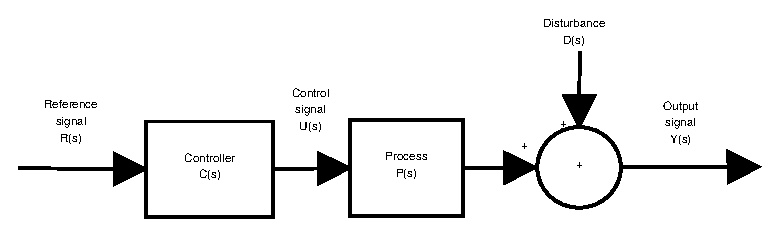
\includegraphics[width=0.7\linewidth]{Open-Loop}
\label{fig:Open-Loop}
\end{figure}
\begin{align*}
	Y = PU = PCR \\
\end{align*}
Remember the example of pouring a glass of water without looking at the glass
\end{itemize}
\end{frame}

\begin{frame}
	\frametitle{A general set-up of a closed loop system}
	\begin{itemize}
		\item We will focus on \underline{closed loop control systems}
		\begin{figure}
\centering
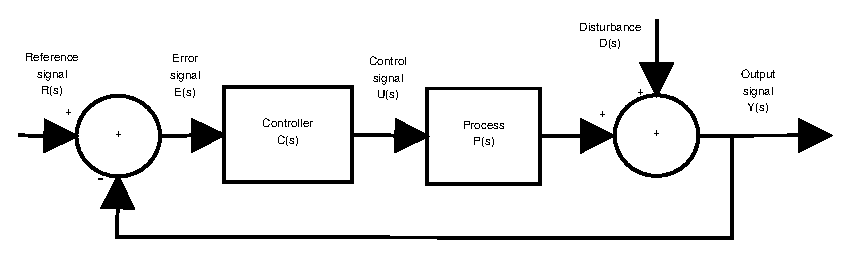
\includegraphics[width=0.7\linewidth]{Closed-Loop}
\label{fig:Closed-Loop}
\end{figure}
\item Example: \href{http://homes.esat.kuleuven.be/~magudelo/_html5/test11.html}{Inverted pendulum}
	\end{itemize}
\end{frame}

\begin{frame}
	\begin{figure}
\centering
\includegraphics[width=0.7\linewidth]{"Inverted Pendulum"}
\caption{Inverted Pendulum}
\label{fig:InvertedPendulum}
\end{figure}
\end{frame}


\begin{frame}
	\frametitle{Concrete Control}
	\begin{itemize}
		\item On-off controller
		\begin{itemize}
			\item Thermostate at home
		\end{itemize}
		\item \textbf{PID controllers, Lead and lag compensators (this course)}
		\begin{itemize}
			\item Cruise-control in your car
		\end{itemize}
		\item More advanced controllers
		\begin{itemize}
			\item STATE-space feedback controllers
			\item Model Predictive Controller (MPC)
			\item Fuzzy Control
			\item Neuro-fuzzy Control
			\item ...
		\end{itemize}
	\end{itemize}
\end{frame}


\section{Control Goals}
\begin{frame}
	\frametitle{What is good control?}
	\begin{itemize}
		\item Before we will start to design control systems we will first focus on the question. What is good control?
		\item It depends on the application
		\begin{itemize}
			\item Stability
			\item Disturbance rejection
			\item Reference tracking (speed)
			\item Sensitivity to errors on model
			\item Etc...
		\end{itemize}
	\end{itemize}
\end{frame}

\begin{frame}
	\frametitle{Examples: stability}
\begin{figure}
\centering
\includegraphics[width=0.7\linewidth]{shuttle}
\caption{Space shuttles are like inverted pendulums. How do you make sure they don't flip over.}
\label{fig:shuttle}
\end{figure}
\end{frame}

\begin{frame}
	\frametitle{Examples: Disturbance rejection}
	\begin{itemize}
		\item Your body will try to keep the temperature in your body as constant as possible. No matter what the outside temperature is. Two people will have almost the same body temperature.
	\end{itemize}
	\begin{figure}
\centering
\begin{minipage}{0.45\textwidth}
\includegraphics[width=0.7\linewidth]{marathon-des-sables}
\caption{Flickr.com, \underline{tent86}, Marathon Des Sables 046}
\label{fig:marathon-des-sables}
\end{minipage}
\centering
\begin{minipage}{0.45\textwidth}
\includegraphics[width=0.7\linewidth]{enduring}
\caption{\underline{Jack Zalium,} Enduring, https://creativecommons.org/licenses/by-nd/2.0/}
\label{fig:enduring}
\end{minipage}
\end{figure}

\end{frame}


\begin{frame}
	\frametitle{Examples: Reference tracking}
	\begin{figure}
\centering
\includegraphics[width=0.7\linewidth]{audi-tracking}
\caption{Audi has a system for automatic driving in traffic jams. The audi will follow the car in front of him at an appropriate distance. \href{https://www.youtube.com/watch?v=Qa_ZSRj0WM0}{youtube}}
\label{fig:audi-tracking}
\end{figure}
\end{frame}

\begin{frame}
	\frametitle{Exercise: name the correct property}
	\begin{figure}
\centering
\includegraphics[width=0.7\linewidth]{ted-drone}
\label{fig:ted-drone}
\end{figure}

\end{frame}


\section{Closed-loop system}

\begin{frame}
	\frametitle{Transfer function of a closed-loop system}
	\begin{flalign*}
		Y(s) - D(s) &= P(s)U(s) \\
		& \text{with } U(s) = C(s)E(s) \\
		Y(s) - D(s) &= P(s)C(s)E(s) \\
		& \text{with} E(s) = R(s) - Y(s) \\
		Y(s) - D(s) &= P(s)C(s) (R(s) - Y(s)) \\
		Y(s) - D(s) &= P(s)C(s)R(s) - P(s)C(s)Y(s) \\
		&\Rightarrow Y(s) = \frac{P(s)C(s)}{1 + P(s)C(s)}R(s) + \frac{1}{1 + P(s)C(s)}D(s)
	\end{flalign*}
	\begin{figure}
\centering
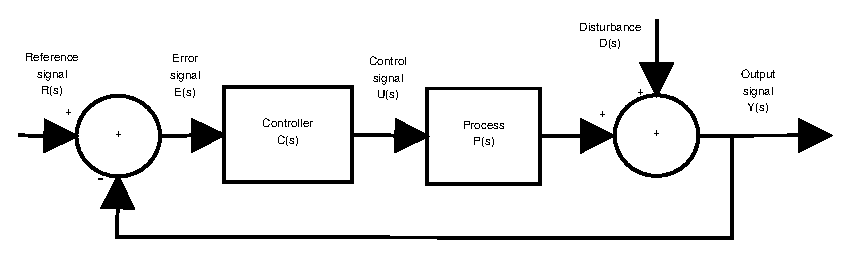
\includegraphics[width=0.7\linewidth]{Closed-Loop}
\label{fig:Closed-Loop2}
\end{figure}

\end{frame}


\begin{frame}
	\frametitle{Transfer function from $R(s)$ to $Y(s)$}
	We define S as the transfer functin from $R(s)$ to $Y(s)$
	\begin{align*}
	S(s) \triangleq \frac{P(s)C(s)}{1 + P(s) C(s)}
	\end{align*}
	This transfer function $S(s)$ will help us to evaluate tracking
	
	Almost perfect tracking: the output $Y(s)$ will follow $R(s)$ very closely $\Rightarrow S(s) \approx 1$
	
\end{frame}


\begin{frame}
	\frametitle{Transfer function from $D(s)$ to $Y(s)$}
	We define $T(s)$ as the transfer function from $D(s)$ to $Y(s)$.
	\begin{align*}
	T(s) \triangleq \frac{1}{1 + P(s)C(s)}
	\end{align*}
	If the disturbance rejection is very good the disturbances will have almost no effect on the output $\Rightarrow T \approx 0$ \\
	
	\[
	\begin{cases}
		\left| S(j\omega) \right| \cong 1 \\
		\left| T(j\omega) \right| \cong 0
	\end{cases}
	\]
	$\Rightarrow  \left| P(j\omega)C(j\omega) \right|$ \textbf{(open loop gain)} is very large. \\
	
	! a large open loop amplification might lead to an unstable system
	
\end{frame}

\begin{frame}
	\frametitle{Model errors}
	\begin{itemize}
		\item In practice, transfer function of $P(s)$ might be unknown. It is important to know what the effect of the model errors will be. Sensitivity and robustness are key-concepts to evaluate these effects.
		\item Sensitivity
		\begin{itemize}
			\item Quantifies the effect of a small perturbation on the model will be on the output. 
		\end{itemize}
		\item Robustness
		\begin{itemize}
			\item This concept refers to bigger changes on the model. A controller is robust if it works properly over a given set of parameters.
		\end{itemize}
	\end{itemize}
\end{frame}

\begin{frame}
	\frametitle{Sensitivity}
	\begin{itemize}
		\item Sensitivity is a measure for the effect of a (small) disturbance on the model (e.g. variations in the process parameters)
		
		\begin{scriptsize}
		\begin{flalign*}
		Y(s) + \Delta Y(s) &= \frac{(P(s) + \Delta P(s))C(s)}{1+(P(s) + \Delta P(s))C(s)}R(s) + \frac{1}{1+(P(s) + \Delta P(s))C(s)}D(s)
		\end{flalign*}
		\end{scriptsize}
		\item Look at the effect on the system without disturbances ($D(s)$=0)
		\begin{flalign*}
			\Delta Y &= \frac{(P+\Delta P)C}{1 + (P + \Delta P)C}R - \frac{PC}{1+PC}R \\
			&= \frac{(P+\Delta P)C(1+PC) - PC - PC(P + \Delta P)C}{(1+(P + \Delta P)C)(1 + PC)}R \\
			&= \frac{\Delta PC}{(1+(P + \Delta P)C)(1+PC)}R \\
			&= Y \frac{\Delta P}{P} \frac{1}{1 + (P + \Delta P)C}
		\end{flalign*}
		
	\end{itemize}
	
\end{frame}


\begin{frame}
	\frametitle{Sensitivity}
	\begin{itemize}
		\item Now take the relative change due to this disturbance of the model and take the limit for $\partial x \rightarrow 0$; this gives the following (measure of the) sensitivity:
		\begin{align*}
			S_P^Y(s) &= \frac{\frac{\partial Y}{Y}(s)}{\frac{\partial P}{P}(s)} = \frac{1}{1 + P(s)C(s)}
		\end{align*}
		\item Again, a very large $\left|P(s)C(s)\right|$ looks like a good choice, but again there is a risk for instability!
		\item Note that the sensitivity can be determined for any parameter
			
	\end{itemize}
\end{frame}